\documentclass[11pt,a4paper]{article}

% Packages
\usepackage[utf8]{inputenc}
\usepackage[T1]{fontenc}
\usepackage[english]{babel}  
\usepackage{amsmath, amssymb}
\usepackage{graphicx}
\usepackage{hyperref}
\usepackage{geometry}
\usepackage{csquotes}
\usepackage[backend=biber,style=authoryear]{biblatex}
\addbibresource{figures/bibliography/references.bib}
\geometry{margin=2.5cm}


    
\title{Community Detection in Bacterial and Viral Networks}
\author{Jonas Ziegler}
\date{\today}

\begin{document}

\maketitle

\begin{abstract}
This paper investigates the community structure of bacterial and viral protein 
similarity networks using modularity-based community detection methods. 
We compare the Louvain and Leiden algorithms and assess the similarity of their 
resulting partitions using the Adjusted Rand Index (ARI).
\end{abstract}

\input{sections/introduction}
\new page
\section{Network Summary Statistics}
\subsection{Basic Metrics}
\section{Similarity Measures for Community Comparison}
\subsection{Adjusted Rand Index (ARI)}
The Adjusted Rand Index (ARI) is a metric that measures the similarity
between two partitions of the same set of nodes. 
A partition refers to the complete division of nodes into clusters.
THE ARI considers all pairs of nodes and evaluates whether each pair is assigned consistently to
the same community or to different communities in both partitions.

The classical Rand Index (RI) evaluates the proportion of node pairs that 
are either placed in both partitions or in different partitions in both clusterings.
However, since random clusterings can also exhibit non-zero agreement,
the ARI corrects this value by adjustion for chance.

Formally, the ARI is defined as:
\begin{equation}
    ARI = \frac{RI - E[RI]}{\max(RI) - E[RI]}
\end{equation}
where $RI$ is the Rand Index, $E[RI]$ is the expected Rand Index for random clusterings, 
and $\max(RI)$ is the maximum possible Rand Index.
The ARI ranges from -1 to 1, where:
\begin{itemize}
    \item 1 indicates perfect agreement between the two partitions,
    \item 0 indicates that the agreement is no better than random,
    \item Negative values indicate less agreement than expected by chance.
\end{itemize}

\subsection{Adjusted Mutual Information (AMI)}
The Adjusted Mutual Information (AMI) is another metric used to compare two partitions 
based on information theory. It measures the mutual information between two clusterings, 
quantifying how much knowing one partition helps to predict the cluster assignments of the other.

Mutual Information (MI) measures the amount of information shared between two partitions.
However, like the RI, MI can be biased by random agreement. The AMI corrects
for this by substracting the expected mutual information under a random model.

The AMI is defined as:
\begin{equation}
    AMI = \frac{MI - E[MI]}{\max(MI) - E[MI]}
\end{equation}
where $MI$ is the Mutual Information, $E[MI]$ is the expected Mutual
Information for random clusterings, and $\max(MI)$ is the maximum possible Mutual Information.
The AMI also ranges from -1 to 1, with similar interpretations as the ARI:
\begin{itemize}
    \item 1 indicates perfect agreement,
    \item 0 indicates agreement no better than random,
    \item Negative values indicate less agreement than expected by chance.
\end{itemize}
\subsection{Comparison of ARI and AMI}
Both ARI and AMI are widely used for evaluating the similarity between two partitions,
however, they differ conceptually and computationally.
The ARI is pair-counting based and  focused on whether pairs of nodes are assigned consistently 
across partitions. It is relatively easy to intepret. However, it can be sensitive
to imbalanced cluster sizes.
On the other hand, AMI is inforamtion-theoretic and evaluates how much information is shared 
between clusterings. It is generally more robust to imbalanced cluster distribution
and performs well when the number of clusters differs between partitions.
The ARI is often preferred when interpretability and pairwise consistency
are important, particulary in case of balanced cluster sizes.

The AMI is advantageous when cluster sizes vary significantly or when
comparing partitions with different numbers of communities.
Due to its information-theoretic nature, it provides a more distribution-sensitive comparison.
Both Indexes are valuable tools for community comparison.
Later in the results section, we will apply both ARI and AMI to compare different
community detection results.



\section{Community Detection Methods}
In this section, we will explore the community detection methods that form
the core of this study.
\subsection{Edge Betweenness}
The edge betweenness method, introduced by Girvan and Newman (2002),
was made to sidestep the shortcomings of traditional community detection methods like 
the hierachical clustering approach. The hierachical clustering method focuses on 
trying to construct a measure that tells us which edges are most central to communities.
Using these measures, it constructs communities by adding the strongest edges
to an initiall empty graph. However, this method has several drawbacks,
such as the fact that it relies on a subjective choice of the similarity measure.
Furthermore, because it tries to build communities by adding edges,
early mistakes made by noise in the data cannot be corrected later on.
The edge betweenness method, on the other hand, removed weak edges from the 
original graph, instead of adding edges.
To find the weak edges of a graoh, Girvan and Newman generalized Freeman's betweenness centrality
to edges. \textcite{newmanandgirvan2002} states if a network contains communities
or groups that are only loosely connected by fe integroup edges, then all shortest paths
different communities must go along one of these few edges. Thus, the edges connecting
communities will have high edge betweenness. By removing these edges, we seperate groups
from one another and so reveal the underlying community structure of the graph.
The algorithm they propose is simply stated as follows:
\begin{enumerate}
  \item Compute the edge betweenness for all edges in the network.
  \item Remove the edge with the highest edge betweenness.
  \item Recalculate the edge betweenness for all edges affected by the removal.
  \item Repeat from step 2 until no edges remain.
\end{enumerate}
The iteration ends when no edges remain, so in praxis, we will have
to decide when to stop the algorithm. This can be done by looking at the modularity of
the network after each iteration and stopping when the modularity is maximized.
This algorithm is computationally expensive, because we have
to recalculate the edge betweenness after each iteration. Making the algorithm
runs in worst-case time $O(m^2n)$, where $m$ is the number of edges and $n$ is 
the number of nodes in the graph.
 So it is tempting to calculate the betweenness of all edges only once and then remove them in order
of decreasing betweenness. However, we find that this approach does not work well,
because if two communities are connected by more than one edge, then there is 
no guarantee that all of the edges will have high betweenness. So by
recalculating betweennesses after the removal of each edge, we can ensure that 
at least one of the remaining edges between two communities will always have high betweenness.

\subsection{Louvain Method}
The Louvain Algorithm 





\section{Data Description}

\subsection{Data Source}

Bacterial proteins for the bac network 
were extracted from full bacterial sequences using Prodigal. 
Viral proteins for the vir network were extracted from viral metagenomic contigs 
after de novo assembly using Prodigal. 

Protein similarity networks were constructed using MMseqs2, a sequence comparison tool 
designed for fast and sensitive large-scale sequence alignment.
Pairwise protein similarities were computed, 
and an edge between two proteins was included in the network if their bit score 
exceeded a threshold of 50.

The resulting networks therefore represent weighted protein similarity 
graphs based on sequence homology. The data originally come from the paper:

\begin{center}
\textit{Whole-Virome Analysis Sheds Light on Viral Dark Matter in Inflammatory Bowel Disease}
\end{center}


\subsection{Descriptive Comparison of Bac and Vir}

The bac network consists of 819 nodes and 88,914 edges, while the vir network
consists of 1,603 nodes and 25,507 edges, meaning the vir network is approximately twice as large
as the bac network. However, the bac network is substantially denser.

The density of the bac network is computed as follows:

\[
\text{Density} = \frac{2E}{N(N-1)} = 
\frac{2 \cdot 88914}{819 \cdot 818} \approx 0.265
\]

meaning that 26.5\% of all possible edges are present in the bac network.

In contrast, the density of the vir network is:

\[
\text{Density} = \frac{2E}{N(N-1)} = 
\frac{2 \cdot 25507}{1603 \cdot 1602} \approx 0.0199
\]

meaning that only 1.99\% of all possible edges are present in the vir network.

The average degree of the bac network is:

\[
\text{Average Degree} = \frac{2E}{N} = \frac{2 \cdot 88914}{819} \approx 217.1
\]

while the average degree of the vir network is:

\[
\text{Average Degree} = \frac{2E}{N} = \frac{2 \cdot 25507}{1603} \approx 31.8
\]

meaning that, on average, bac proteins are approximately seven times more similar to other proteins
than vir proteins.

Based on the substantially higher average connectivity of the bacterial network, 
its degree distribution is expected to be comparatively homogeneous and 
concentrated around higher degree values. The dense connectivity suggests 
the presence of strongly interconnected subclusters, potentially approaching 
quasi-complete structures within communities.

In contrast, the viral network is expected to exhibit a more heterogeneous and 
potentially heavy-tailed degree distribution. 
Such a structure would be characterized by a small number of highly 
connected hub nodes and a large proportion of weakly connected proteins, 
reflecting a sparse and modular topology.

By computing the degree distribution of both networks,
the structural differences can be visualized using a histogram:

\begin{center}
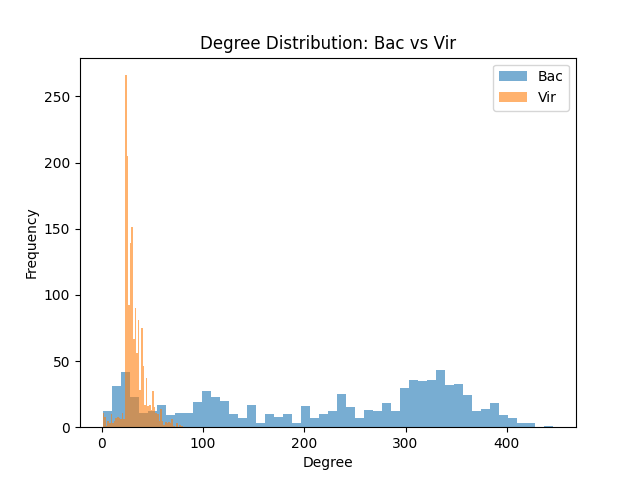
\includegraphics[width=0.8\textwidth]{Figures/data_description/data_distribution_comparison.png}
\end{center}

The histogram clearly shows that the bacterial network is characterized by 
substantially higher node degrees compared to the viral network. 
While the viral network exhibits a strong concentration of low-degree nodes, 
the bacterial network displays a broad distribution extending to very high degree values.
This indicates a much denser and more interconnected structure in the bacterial network,
whereas the viral network appears sparse and modular.

\subsection{Network Construction}

The networks are constructed based on sequence similarity between proteins.
Nodes represent proteins, and edges represent sequence similarity between them.
The weight of each edge is calculated using the bit score,
which is a normalized measure of sequence similarity derived from 
the raw alignment score.

The bit score is computed using the following formula:

\[
S' = \frac{\lambda S - \ln K}{\ln 2}
\]

where \(S\) is the raw alignment score, \(\lambda\) and \(K\) 
are statistical parameters derived from the scoring system used in the sequence alignment,
and \(\ln\) denotes the natural logarithm.

The bit score provides a standardized way to compare sequence 
similarities across different alignments, allowing for a more 
meaningful interpretation of the edge weights in the 
context of protein similarity networks.


\section{Experimental Setup}

\subsection{Implementation}

After describing the data and the community detection methods, 
we now apply these methods to analyze the bacterial 
and viral protein similarity networks.

All analyses were implemented in Python. 
Graph construction and basic network measures were computed using the 
NetworkX library, while the Leiden algorithm was executed 
using the \texttt{leidenalg} package in combination with \texttt{igraph}.

The full source code is publicly available at:
\url{https://github.com/j0nascz/Paper_SMNCA.git}

\subsection{Evaluation Criteria}

The goal of this analysis is to compare the three community detection methods
(Edge Betweenness, Louvain, and Leiden) in terms of their ability
to identify meaningful communities in the bac and vir networks.

However, we cannot apply the edge betweenness approach proposed by Girvan and Newman,
as it is computationally infeasible for networks of this size.
Consequently, we focus on comparing the Louvain and Leiden methods.

The evaluation is based on a pairwise comparison of the resulting partitions 
using the Adjusted Rand Index (ARI) and the Adjusted Mutual Information (AMI).

\section{Results}

\subsection{Method Comparison}

The results of the Leiden and Louvain algorithms applied to the Bac and Vir networks are summarized in the following table:

\begin{table}[htbp]
\centering
\caption{Community detection results for bacterial and viral networks.}
\label{tab:community_results}
\begin{tabular}{lcccc}
\hline
Dataset & Method & \# Communities & Modularity & Runtime (s) \\
\hline
Bac & Louvain & 5  & 0.374 & 0.340 \\
Bac & Leiden  & 6  & 0.333 & 0.017 \\
Vir & Louvain & 23 & 0.892 & 0.136 \\
Vir & Leiden  & 23 & 0.884 & 0.007 \\
\hline
\end{tabular}
\end{table}

For the Bac network, the Louvain algorithm identified 5 communities, 
whereas the Leiden algorithm detected 6 communities.
The slight increase in the number of communities produced by Leiden suggests a 
refinement of the partition obtained by Louvain. This behavior is consistent with the theoretical properties
of the Leiden algorithm, which aims to ensure better-connected and more internally coherent communities.

In terms of modularity, Louvain achieved a value of approximately 0.374,
while Leiden reached approximately 0.333. 
The higher modularity value for Louvain in the bacterial network suggests that 
Louvain is more effective at optimizing the modularity objective in this specific case.
This indicates that, although Leiden produces a slightly more refined partition, 
the Louvain partition achieves stronger optimization of the modularity objective under the given settings.

For the Vir network, which has approximately twice as many nodes as the Bac network,
both Louvain and Leiden identified 23 communities in the viral network.
The strong agreement between the two methods indicates that the underlying community 
structure is clearly defined and does not depend strongly on the specific optimization strategy.

In terms of modularity, Louvain achieved a value of approximately 0.892,
while Leiden obtained approximately 0.884.
Although Louvain reaches a slightly higher modularity score,
the difference between the two methods is small. 
This indicates that both algorithms produce partitions of very similar quality 
with respect to modularity optimization.

As expected, the runtime of the Louvain algorithm was higher than that of the Leiden algorithm in both networks.
For the Bac network, Louvain required approximately 0.340 seconds, while Leiden required approximately 0.017 seconds.
For the Vir network, Louvain required approximately 0.136 seconds, while Leiden required approximately 0.007 seconds.

This difference in runtime can be attributed to more efficient local moving, a better-structured
aggregation phase, and faster convergence of the Leiden algorithm compared to Louvain, 
especially in larger networks.

\subsection{ARI}

The Adjusted Rand Index (ARI) further confirms the strong agreement between Louvain and Leiden. 
For the viral network, the ARI is approximately 0.979, 
indicating an almost identical partitioning of the network by both algorithms.

For the bacterial network, the ARI is slightly lower at approximately 0.958,
yet it still reflects a very high degree of similarity. 
The minor difference can be attributed to the additional community detected by Leiden, 
which suggests a small refinement of the Louvain partition rather than a 
fundamentally different community structure.

Overall, the high ARI values demonstrate that both methods 
produce highly consistent community assignments across both datasets.

\subsection{Stability of Communities}

The observed differences between the Bac and Vir networks can be attributed to their fundamentally
different structural organization. The bacterial network is denser and more strongly connected,
indicating the presence of tightly interconnected protein communities.
Such dense connectivity implies that many proteins are linked across different regions of
the network, resulting in a cohesive structure with numerous inter-community connections.
In contrast, the viral network is sparser and contains a larger proportion of weakly
connected nodes. Connections between modules are less frequent, leading to sharper boundaries
between communities.
These structural differences are directly reflected in the modularity values. Modularity
measures the extent to which connections are concentrated within communities rather than 
between them.
In the dense bacterial network, the abundance of cross-community edges reduces
the contrast between intra- and inter-community connectivity. As a result, the modularity 
remains comparatively lower.
In the sparse viral network, the clear separation between communities leads to a higher modularity score,
as the majority of connections are concentrated within communities rather than between them.
Thus, the difference in modularity between the two datasets does not indicate better algorithmic 
performance on the viral network, but rather reflects the intrinsic topological differences between 
a densely interconnected graph and a more clearly segmented modular structure.





\section{Discussion}

\subsection{Differences Between Bac and Vir Networks}

The observed differences in community structure between the Bac and Vir networks
can primarily be attributed to their underlying structural organization.
The Bac network is characterized by a higher edge density and stronger overall connectivity,
suggesting the presence of tightly interconnected protein communities.
In contrast, the Vir network exhibits a sparser structure with a larger 
proportion of weakly connected nodes.

\subsection{Which Method Is More Stable}

Stability in community detection refers to the robustness 
of identified partitions under methodological variation.
The high agreement between Louvain and Leiden in both networks, as indicated by the ARI values,
suggests that both methods produce stable community assignments.
This reinforces confidence in the reliability of the detected communities.

\subsection{Resolution Limit Problem}

An important limitation of modularity-based community detection methods, such as Louvain and Leiden,
is the resolution limit problem. Modularity optimization may fail to 
detect smaller but well-defined communities if merging them with larger groups
results in a higher overall modularity score.

This limitation is particularly relevant for dense networks such as Bac, where small modules
may be overlooked in favor of larger communities, leading to a
less accurate representation of the true community structure.

Although the Leiden algorithm is designed to produce better-connected communities, 
it is not immune to the resolution limit problem.
Therefore, the detected partitions should be interpreted as optimal with respect to the 
chosen resolution parameter rather than as uniquely defined ground-truth communities.
\section{Conclusion}

\subsection{Summary of Findings}

This study compared the performance of the Louvain and Leiden community detection algorithms
on two biological networks: a bacterial protein–protein interaction network (Bac) 
and a viral protein–protein interaction network (Vir). 
The results, evaluated using the Adjusted Rand Index (ARI), show that both methods identify
highly consistent community structures across both networks. 
This is also reflected in the similar number of communities detected and the comparable modularity scores.

A notable difference observed in this study is that the runtime of
the Leiden algorithm was significantly lower than that of the Louvain algorithm.
This efficiency gain is particularly evident in the larger viral network, 
where Leiden's runtime was approximately an order of magnitude faster than Louvain's.

Overall, the findings suggest that both Louvain and Leiden are 
effective methods for community detection in biological networks.

\subsection{Outlook and Future Work}

This study was originally intended to include an evaluation of the edge-betweenness 
algorithm by Girvan and Newman. However, due to runtime limitations, it was not possible
to include it in the analysis. For future work, it may be worthwhile to explore
ways to improve the computational efficiency of the algorithm. At present, it runs in time 
$O(n^3)$ on sparse graphs, which makes it infeasible for larger networks.

Future research could also further investigate intra-method stability by varying the
resolution parameter in both the Louvain and Leiden algorithms.
Additionally, alternative quality functions beyond modularity could
be explored to address potential limitations such as the resolution limit problem.
Finally, integrating biological validation of detected communities would provide further 
insight into the functional relevance of the identified modular structures.


\printbibliography
\end{document}

